\documentclass{article}
\usepackage[utf8]{inputenc}
\usepackage[parfill]{parskip}
\usepackage{float}
\usepackage{amsmath}
\usepackage{amsfonts}
\usepackage{amssymb}
\usepackage{tikz}
\usepackage{pgfplots}
\usepgfplotslibrary{fillbetween}
\usetikzlibrary{patterns}
\usepackage{color}
\usetikzlibrary{decorations.markings}
\usepackage{mhchem}
\usepackage[makeroom]{cancel}
\usepackage{hyperref}
\hypersetup{
    colorlinks=true,
    linkcolor=blue,
    filecolor=magenta,
    urlcolor=cyan,
}
\urlstyle{same}

\usepackage{biblatex}
\addbibresource{citations.bib}


\title{\vspace{-2cm}}
\author{MedicinalYoyos}

\begin{document}

\maketitle

\section*{Intro}

View the most up-to-date version of this doc \href{https://www.overleaf.com/read/rgykqvzvfnvv}{here}.

View it on GitHub \href{https://github.com/Yoyomanzoor/BiochemPassage/blob/main/main.pdf}{here}.

Steady-state assumptions and defining $K_M$.

\begin{center}
\ce{
{E} + {S} <=>[k_1][k_{-1}]
\ce{ES} <=>[k_2][k_{-2}]
\ce{EP} <=>[k_3][k_{-3}]
\ce{E} + {P}
}
\end{center}

\begin{equation}
    k_{cat} = \frac{k_2k_3}{k_2 + k_3}
\end{equation}

\begin{align*}
    k_3 &>> k_2 \\
    k_{cat} &= \frac{k_2k_3}{\cancel{k_2} + k_3} \\
    &= \frac{k_2\cancel{k_3}}{\cancel{k_3}} \nonumber \\
    \implies k_{cat} &\approx k_2
\end{align*}

Thus,

\begin{center}
\ce{
{E} + {S} <=>[k_1][k_{-1}]
\ce{ES} ->[k_{cat}]
\ce{E} + {P}
}
\end{center}

\begin{equation}
    K_M = \frac{k_{-1} + k_{cat}}{k_1}
\end{equation}

\begin{equation}
    V = \frac{V_{max}[S]}{K_M + [S]}
\end{equation}

\begin{equation}
    V_{max} = k_{cat} [E_T]
\end{equation}

\begin{equation}
    E_T = [E] + [ES]
\end{equation}

\begin{equation}
    \text{Catalytic~efficiency} = \frac{k_{cat}}{K_m}
\end{equation}

% \begin{equation}
%     \frac{d[ES]}{dt} = k_1[E][S] - (k_{-1}[ES] + k_{cat}[ES])
% \end{equation}

\pagebreak

M-M graph with the equation: $V=\frac{3[S]}{0.5+[S]}$

\begin{center}
\begin{tikzpicture}
\begin{axis}[
         axis equal,
         %domain=-3:3,
         % grid,
         % grid style={dashed,gray!30},
         smooth,
         xmin=0, xmax=8,
         ymin=0, ymax=3.5,
         axis lines=middle,
         xlabel=$Conc.~S$,
         xlabel style={at={(axis description cs:0.5,0)},anchor=north},
         xtick={0,...,7},
         ylabel=$V$,
         ylabel style={at={(axis description cs:-0.2,.5)},anchor=south},
         ytick={0,...,3},
         samples=100,
         legend style={at={(1,1)},xshift=0cm,anchor=north east,nodes=right,fill=none}
 ]
 \addplot[black, name path=f1,mark=none,domain=0:8] {(3*x)/(0.5+x)}
 node{};
 \draw[dashed] (axis cs:0.5,0) -- (axis cs:0.5,3);
\end{axis}
\end{tikzpicture}
\end{center}

M-M graphs with the following parameters:

\begin{itemize}
    \item In black: $V=\frac{3[S]}{0.5+[S]}$
    \item In \textcolor{red}{red}: $V=\frac{3[S]}{1+[S]}$, an example of competitive inhibition.
    \item In \textcolor{blue}{blue}: $V=\frac{1.5[S]}{0.5+[S]}$, an example of noncompetitive inhibition.
    \item In \textcolor{green}{green}: $V=\frac{1.5[S]}{0.25+[S]}$, an example of uncompetitive inhibition.
\end{itemize}

\begin{center}
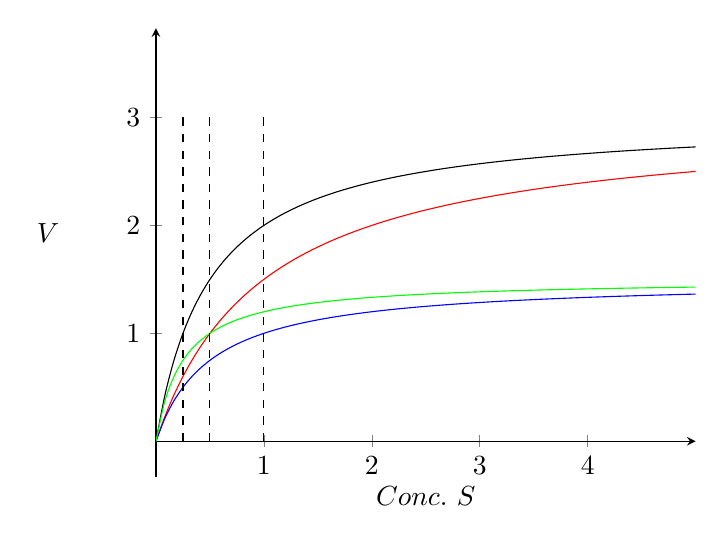
\begin{tikzpicture}
\begin{axis}[
         axis equal,
         %domain=-3:3,
         % grid,
         % grid style={dashed,gray!30},
         smooth,
         xmin=0, xmax=5,
         ymin=0, ymax=3.5,
         axis lines=middle,
         xlabel=$Conc.~S$,
         xlabel style={at={(axis description cs:0.5,0)},anchor=north},
         xtick={0,...,4},
         ylabel=$V$,
         ylabel style={at={(axis description cs:-0.2,.5)},anchor=south},
         ytick={0,...,3},
         samples=100,
         legend style={at={(1,1)},xshift=0cm,anchor=north east,nodes=right,fill=none}
 ]
 \addplot[black, name path=f1,mark=none,domain=0:8] {(3*x)/(0.5+x)}
 node{};
 \addplot[red, name path=f1,mark=none,domain=0:8] {(3*x)/(1+x)}
 node{};
 \addplot[blue, name path=f1,mark=none,domain=0:8] {(1.5*x)/(0.5+x)}
 node{};
 \addplot[green, name path=f1,mark=none,domain=0:8] {(1.5*x)/(0.25+x)}
 node{};
 \draw[dashed] (axis cs:1,0) -- (axis cs:1,3);
 \draw[dashed] (axis cs:0.5,0) -- (axis cs:0.5,3);
 \draw[dashed] (axis cs:0.25,0) -- (axis cs:0.25,3);
\end{axis}
\end{tikzpicture}
\end{center}

\pagebreak

Deriving Lineweaver-Burk

\begin{equation*}
    V = \frac{V_{max}[S]}{K_M + [S]}
\end{equation*}

Inverse:

\begin{align}
    \frac{1}{V} &= \frac{K_M + [S]}{V_{max}[S]} \\
    &= \frac{K_M}{V_{max}[S]} + \frac{[S]}{V_{max}[S]} \\
    &= \frac{K_M}{V_{max}}(\frac{1}{[S]}) + \frac{1}{V_{max}}
\end{align}

This is just a fancy $y = mx+b$!

\begin{center}
\begin{tikzpicture}
\begin{axis}[
         axis equal,
         %domain=-3:3,
         % grid,
         % grid style={dashed,gray!30},
         smooth,
         xmin=-2.5, xmax=1,
         ymin=0, ymax=0.5,
         axis lines=middle,
         y=0.5cm/1.5,
         x=0.1cm,
         xlabel=$\frac{1}{[S]}$,
         xlabel style={at={(axis description cs:1,0.2)},anchor=north},
         xtick={-2,...,0},
         ylabel=$\frac{1}{V}$,
         ylabel style={at={(axis description cs:0.75,0.75)},anchor=south},
         % ytick={0,...,0.5},
         samples=100,
         legend style={at={(1,1)},xshift=0cm,anchor=north east,nodes=right,fill=none}
 ]
 \addplot[black, name path=f1,mark=none,domain=-2:1] {((0.5*x)/3)+(1/3)}
 node{};
\end{axis}
\end{tikzpicture}
\end{center}

\pagebreak

These are the same equations as earlier, translated to Lineweaver-Burk.

\begin{itemize}
    \item In black: $\frac{1}{V} = \frac{0.5}{3}(\frac{1}{[S]}) + \frac{1}{3}$ (M-M: $V=\frac{3[S]}{0.5+[S]}$)
    \item In \textcolor{red}{red}: $\frac{1}{V} = \frac{1}{3}(\frac{1}{[S]}) + \frac{1}{3}$ (M-M: $V=\frac{3[S]}{1+[S]}$) - competitive inhibition.
    \item In \textcolor{blue}{blue}: $\frac{1}{V} = \frac{0.5}{1.5}(\frac{1}{[S]}) + \frac{1}{1.5}$ (M-M: $V=\frac{1.5[S]}{0.5+[S]}$) - noncompetitive inhibition.
    \item In \textcolor{green}{green}: $\frac{1}{V} = \frac{0.25}{1.5}(\frac{1}{[S]}) + \frac{1}{3}$ (M-M: $V=\frac{1.5[S]}{0.25+[S]}$) - uncompetitive inhibition.
\end{itemize}

\begin{center}
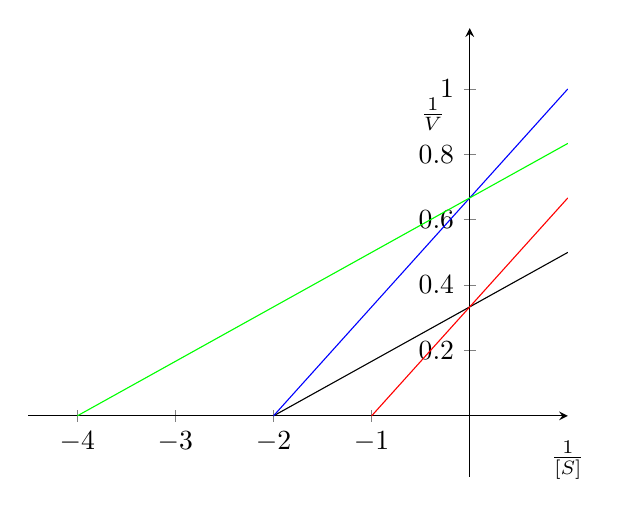
\begin{tikzpicture}
\begin{axis}[
         axis equal,
         %domain=-3:3,
         % grid,
         % grid style={dashed,gray!30},
         smooth,
         xmin=-4.5, xmax=1,
         ymin=0, ymax=1,
         axis lines=middle,
         y=0.5cm/1.5,
         x=0.1cm,
         xlabel=$\frac{1}{[S]}$,
         xlabel style={at={(axis description cs:1,0.1)},anchor=north},
         xtick={-4,...,0},
         ylabel=$\frac{1}{V}$,
         ylabel style={at={(axis description cs:0.75,0.75)},anchor=south},
         % ytick={0,...,0.5},
         samples=100,
         legend style={at={(1,1)},xshift=0cm,anchor=north east,nodes=right,fill=none}
 ]
 \addplot[black, name path=f1,mark=none,domain=-2:1] {((0.5*x)/3)+(1/3)}
 node{};
 \addplot[red, name path=f1,mark=none,domain=-1:1] {((1*x)/3)+(1/3)}
 node{};
 \addplot[blue, name path=f1,mark=none,domain=-2:1] {((0.5*x)/1.5)+(1/1.5)}
 node{};
 \addplot[green, name path=f1,mark=none,domain=-4:1] {((0.25*x)/1.5)+(1/1.5)}
 node{};
\end{axis}
\end{tikzpicture}
\end{center}

\pagebreak

\section*{Passage (Question 1-6)}
% The effect of food on skin pigmentation.

% Melanocytes are pigment-producing cells in the basal layer of the epidermis. They produce and store melanin 

% Melanocytes, located in the basal layer of the epidermis, produce and store melanin in melanosomes. Melanosomes are organelles bound by a phopholipid bilayer that transport melanin throughout the epidermis. The production of melanin is as follows: tyrosine is oxidized by tyrosinase to form L-DOPA. L-DOPA is further oxidized by tyrosinase to form Dopaquinone. Dopaquinone undergoes a series of reactions to form melanin.

% The production of melanin is as follows: tyrosine is oxidized by tyrosinase to form L-DOPA. L-DOPA is further oxidized by tyrosinase to form Dopaquinone. Dopaquinone undergoes a series of reactions to form melanin.


Melanin is a pigment produced by melanocytes in the basal layer of the epidermis. It is the primary determinant of skin color in humans. Melanocytes are dendritic in shape and produce and store melanin in melanosomes. Melanosomes are phospholipid-bound organelles that transport and deposit melanin throughout the epidermis. An image of this process is shown below.

\begin{figure}[h]
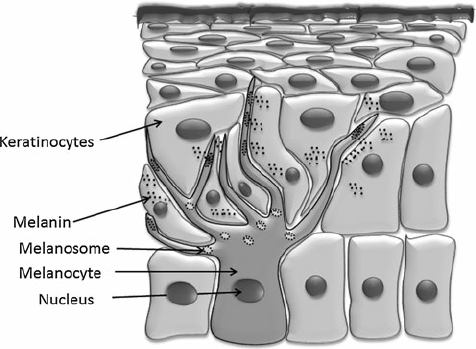
\includegraphics[scale=0.4]{melanocyte.png}
\centering
\end{figure}

Tyrosinase is an important oxidase in the production of melanin. Tyrosine is oxidized by tyrosinase to form L-DOPA. L-DOPA is further oxidized by tyrosinase to form Dopaquinone. Dopaquinone undergoes a series of reactions to form melanin.

A group of researchers were interested in whether citrus essential oils have an effect on tyrosinase. From the oils of 13 citrus fruits, they found three inhibitory extracts, citral, myrcene, and kojic acid. The results of an enzyme assay for tyrosinase on the substrate L-DOPA are shown below.

\begin{figure}[H]
\centering
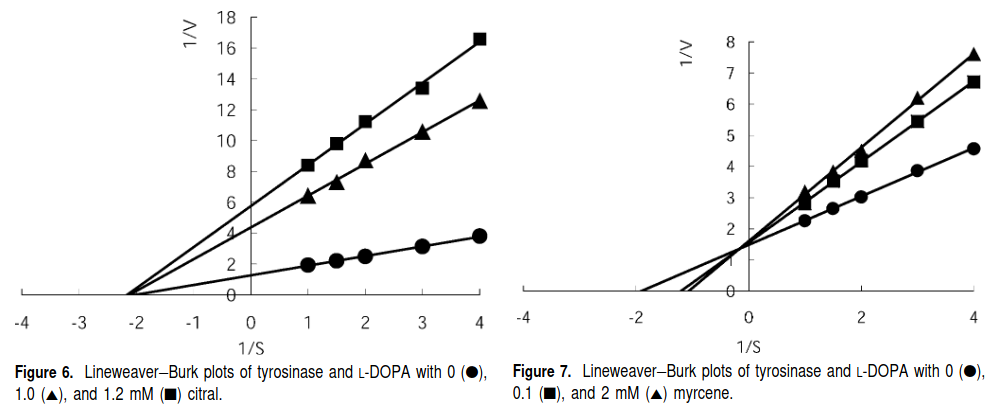
\includegraphics[width=\textwidth]{fig.png}
\end{figure}

\vfill

\footnotesize{Study and figures pulled from \textit{Matsuura, R. et al.} \cite{pmid16536612}. Please note details of the study were altered. to suit the passage.}

\section*{Questions}
\begin{enumerate}
    \item What are the likely reactants for the first step of melanin production mentioned in the passage?
    \begin{enumerate}
        \item L-tyrosine + water
        \item L-tyrosine + an electron source
        \item D-tyrosine + water
        \item L-tyrosine + NADH$^+$+H$^+$
    \end{enumerate}
    
    \item Which of the following are likely to cause depigmented skin?
    
    I. An autoimmune disease where melanocytes are destroyed by macrophages.

    II. An ointment that increases the production of L-DOPA.

    III. A medicine that reduces the Vmax of all oxidases.
    
    \begin{enumerate}
        \item I only
        \item I and II
        \item I and III
        \item I, II, and III
    \end{enumerate}

    \item What type of inhibitor is citral?
    \begin{enumerate}
        \item competitive inhibitor
        \item uncompetitive inhibitor
        \item noncompetitive inhibitor
        \item allosteric inhibitor
    \end{enumerate}

    \item Tinea versicolor is a disease where a yeast that produces azelaic acid grows on the skin. Azelaic acid is a competitive inhibitor of tyrosinase. Which of the following is true?
    \begin{enumerate}
        \item $K_M$ of tyrosinase would increase as the concentration of azelaic acid increases.
        \item Tyrosinase will have a lower catalytic efficiency in the presence of azelaic acid.
        \item $V_{max}$ of tyrosinase will decrease due to azelaic acid.
        \item Azelaic acid will cause negative cooperativity in tyrosinase.
    \end{enumerate}

    \item What is the likely mechanism for the transport of melanin?
    \begin{enumerate}
        \item Kinesin-mediated anterograde transport.
        \item Actin-mediated anterograde transport.
        \item Kinesin-mediated retrograde transport.
        \item Actin-mediated retrograde transport.
    \end{enumerate}

    \item Kojic acid is found to be a mixed inhibitor. Assuming there is unlimited large supply of subtrate, will the reaction velocity of tyrosinase be faster in the presence of myrcene or kojic acid?
    \begin{enumerate}
        \item Kojic acid because $V_{max}$ is decreased by myrcene.
        \item Kojic acid because $V_{max}$ is increased by kojic acid.
        \item Myrcene because $K_M$ of tyrosinase is lowered by myrcene.
        \item Myrcene because $V_{max}$ of tyrosinase is lowered by kojic acid.
    \end{enumerate}
\end{enumerate}

% Matsuura, R., Ukeda, H., \& Sawamura, M. (2006). Tyrosinase inhibitory activity of citrus essential oils. \textit{Journal of Agricultural and Food Chemistry}, \textit{54}(6), 2309–2313. https://doi.org/10.1021/jf051682i

\pagebreak

\section*{Answer Key}

\begin{enumerate}
    \item B
    \item C
    \item C
    \item A
    \item A
    \item D
\end{enumerate}

\section*{Explanations}

Alas, it is summer and the days are long. Yet somehow my time is short, and I have not found the time to write out answer explanations.

Discussion on tyrosine hydroxylase vs tyrosinase https://jn.nutrition.org/article/S0022-3166(22)15174-6/fulltext

\section*{Bonus Questions}

These are ideas for questions I have not finished, so maybe come back here once I finish them!

\begin{enumerate}
    \item Mutations in the gene that encodes tyrosinase is a common cause for albinism and is inherited in an autosomal recessive manner.  Suppose a mutation alters the open reading frame of the TYR gene, which produces tyrosinase. How would this affect the 
    \item Mut on ORF of TYR, something about destruction in ERAS
    \item Something about Malassezia Furfur
    \item Something about dopamine vs melanin
    \item T. gondii affect on tyrosine hydroxylase efficiency or vaccination https://pubmed.ncbi.nlm.nih.gov/32244791/
    \item Tinea versicolor is a disease where a yeast that produces azelaic acid grows on the skin. Azelaic acid is a competitive inhibitor of tyrosinase. Which of the following is true?
    \begin{enumerate}
        \item $K_M$ of tyrosinase would increase as the concentration of azelaic acid increases.
        \item Tyrosinase will have a lower catalytic efficiency in the presence of azelaic acid.
        \item $V_{max}$ of tyrosinase will decrease due to azelaic acid.
        \item Azelaic acid will cause negative cooperativity in tyrosinase.
    \end{enumerate}
\end{enumerate}

\printbibliography

\end{document}

